\thispagestyle{lichsutoanhocnone}
\pagestyle{lichsutoanhoc}
\graphicspath{{../lichsutoanhoc/pic/}}
\everymath{\color{lichsutoanhoc}}
\blfootnote{$^*$\color{lichsutoanhoc}Bản gốc có thể xem tại \href{https://media.nature.com/original/magazine-assets/d41586-018-00513-8/d41586-018-00513-8.pdf}{\color{lichsutoanhoc}The Fields Medal should return to its roots. Nature $553$, $18$ January $2018$, pp. $271-273'$}}
\blfootnote{$^2$\color{lichsutoanhoc}Đại học Osnabr\"uck.}
\begingroup
\AddToShipoutPicture*{\put(0,616){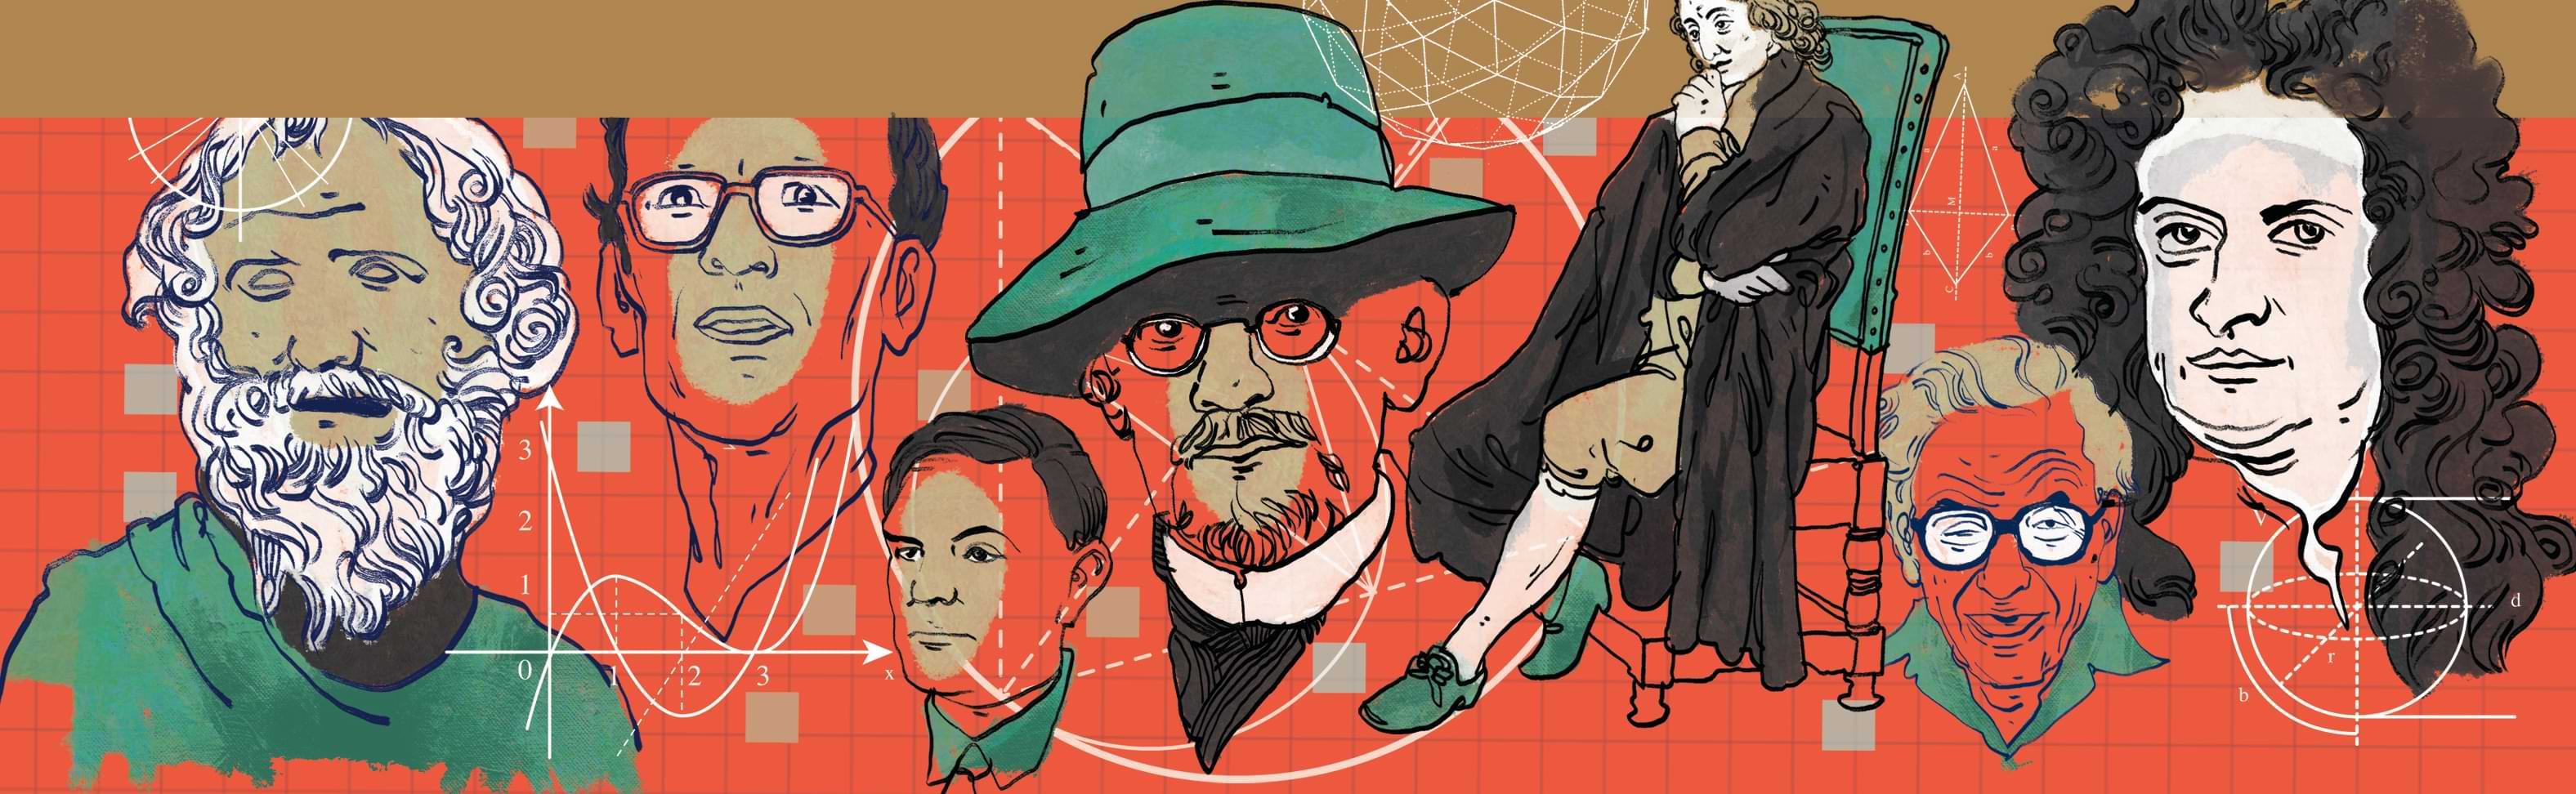
\includegraphics[width=19.3cm]{../bannerlichsu}}}
\AddToShipoutPicture*{\put(90,490){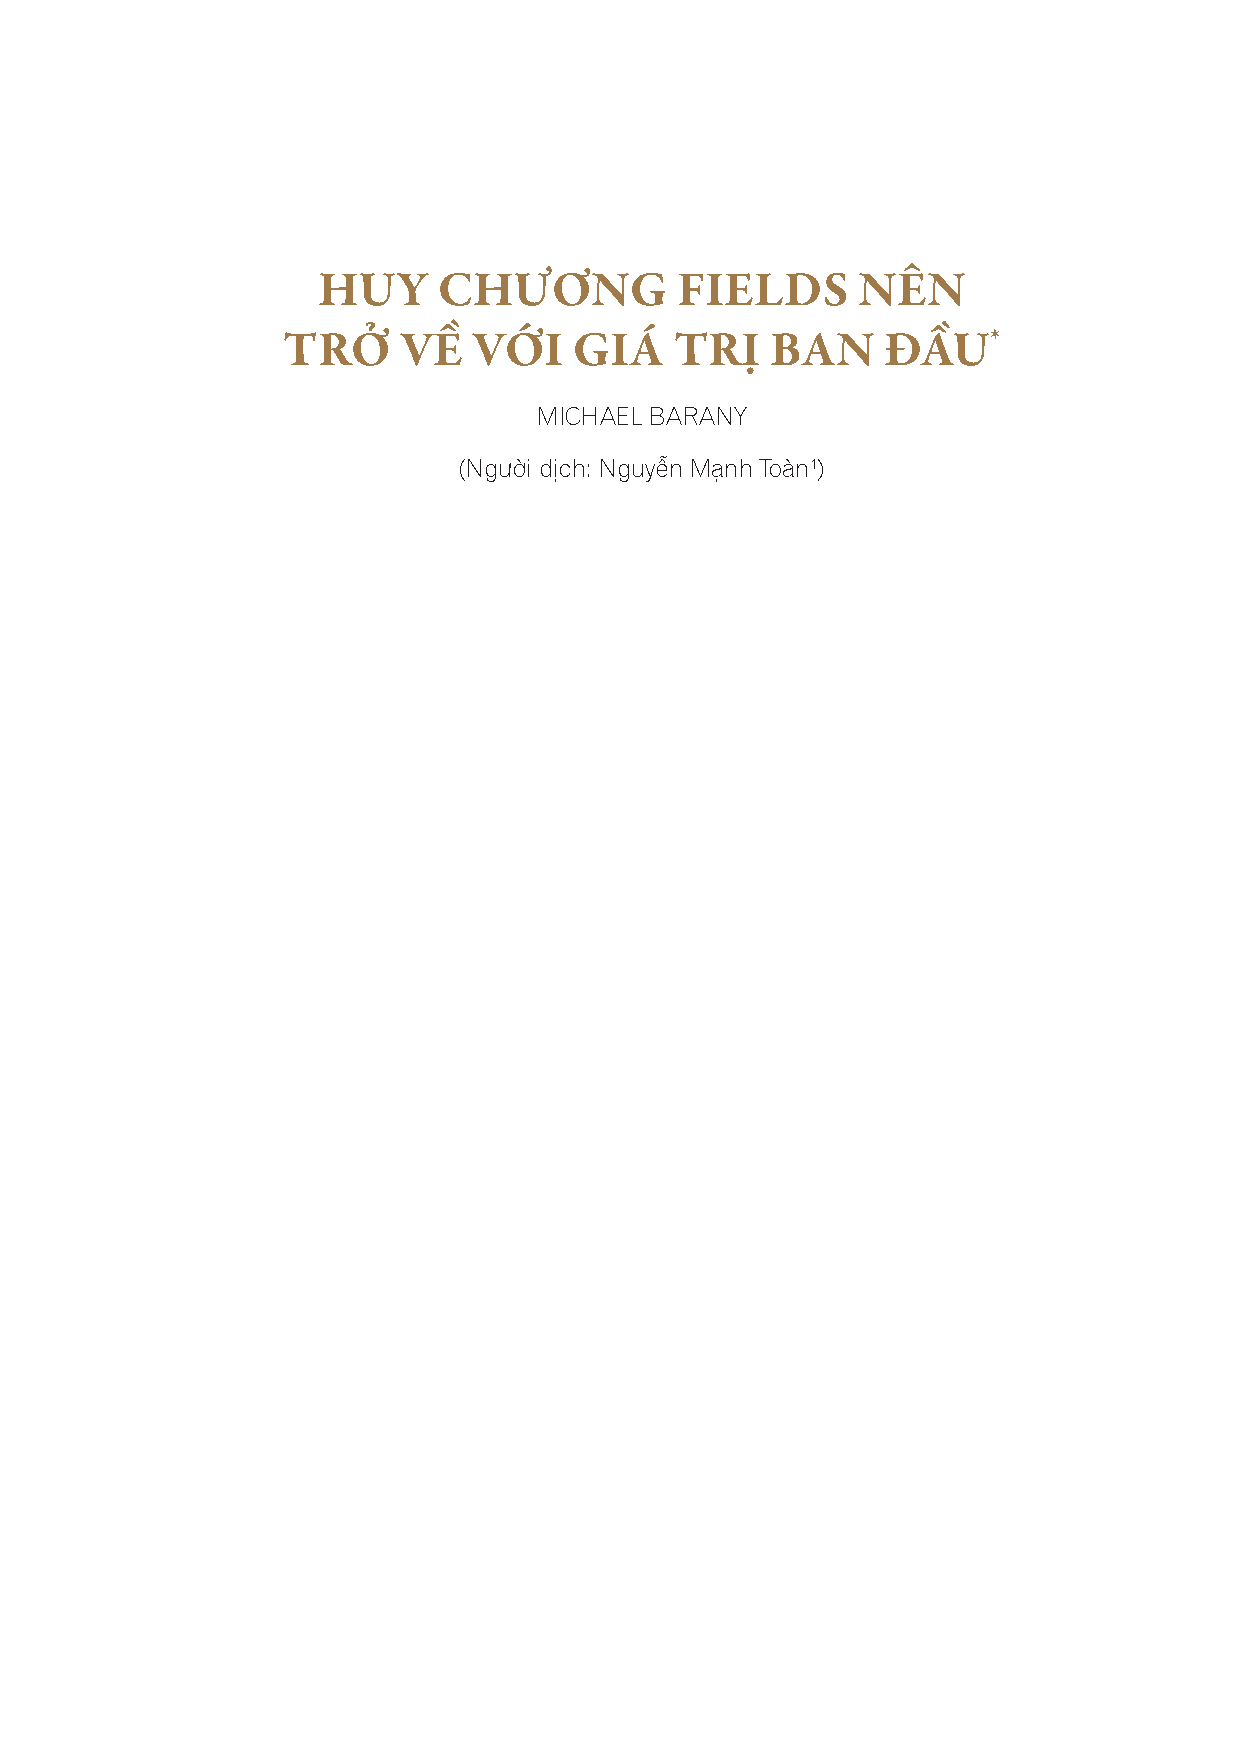
\includegraphics[scale=1]{../tieude1.pdf}}}
\centering
\endgroup

\vspace*{215pt}

\begin{multicols}{2}
	\textit{
		Những hồ sơ bị lãng quên về giải thưởng danh giá nhất của toán học lưu giữ những bài học cho tương lai của ngành này, lập luận của nhà sử học Michael Barany.}
	\begin{figure}[H]
		\vspace*{-5pt}
		\centering
		\captionsetup{labelformat= empty, justification=centering}
		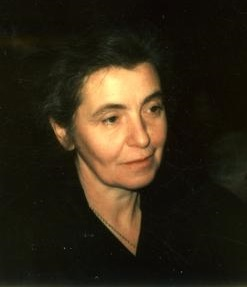
\includegraphics[width= 0.85\linewidth]{OlgaLadyzhenskaya}
		\caption{\small\textit{\color{lichsutoanhoc}Olga Ladyzhenskaya lọt vào danh sách rút gọn Huy chương Fields năm $1958$. Nguồn: Karl Nickel -- Oberwolfach Photo Collection.}}
		\vspace*{-10pt}
	\end{figure}
	Cũng giống như huy chương Thế vận hội hay cúp vàng bóng đá thế giới, giải thưởng danh giá nhất ngành Toán học chỉ được trao bốn năm một lần. Ngay từ bây giờ, các khoa toán trên toàn thế giới đang xôn xao với những tin đồn, bởi $2018$ là năm của huy chương Fields.
	\vskip 0.1cm
	Trong niềm hân hoan hướng tới buổi lễ công bố của năm nay, tôi đã nhìn về quá khứ với sự quan tâm thậm chí còn lớn hơn. Trong các tập tài liệu lưu trữ bị lãng quên từ lâu, tôi đã tìm thấy những chi tiết về các bước ngoặt trong quá khứ của huy chương này mà theo quan điểm của tôi, là bài học cho những người đang cân nhắc sẽ công nhận ai vào tháng $8$ tới tại Đại hội toán học thế giới $2018$ (International Congress of Mathematicians--ICM) ở Rio de Janeiro ở Brazil, và cả sau đó~nữa.
	\vskip 0.1cm
	Từ cuối những năm $1960$, huy chương Fields đã được so sánh một cách rộng rãi với giải Nobel, nơi không có hạng mục nào dành cho toán học [$1$]. Trên thực tế, cả hai rất khác nhau về thủ tục, tiêu chí, tiền thưởng và nhiều mặt khác nữa. Đặc biệt, giải Nobel thường được trao cho những nhà khoa học lỗi lạc, những người được vinh danh thường hàng thập kỷ sau những cống hiến. Ngược lại, những người nhận huy chương Fields lại ở độ tuổi mà, trong hầu hết các ngành khoa học, một sự nghiệp đầy hứa hẹn chỉ mới vừa cất cánh.
	\vskip 0.1cm
	Ý tưởng trao một giải thưởng danh giá cho những ngôi sao đang lên, những người đã tạo được dấu ấn lớn khi còn khá trẻ -- bằng sự xuất sắc, may mắn và hợp thời -- là một sự tình cờ của lịch sử. Nó không phản ánh bất kỳ mối liên hệ đặc biệt nào giữa toán học và tuổi trẻ -- một truyền thuyết\footnote[3]{\color{lichsutoanhoc}Nhà toán học Godfrey Harold Hardy từng nói: ``Toán học, hơn bất kỳ lĩnh vực khoa học và nghệ thuật nào, là cuộc chơi của những người trẻ tuổi".} không được các số liệu xác nhận [$2$, $3$]. Như một số nhà toán học đã nhận ra từ lâu [$4$], chính sự tình cờ này đã làm tổn hại đến toán học. Nó củng cố những định kiến trong ngành cũng như trong quan điểm của công chúng về công việc, con đường sự nghiệp, các giá trị trí tuệ và xã hội của các nhà toán học. Tất cả $56$ người đoạt giải cho đến nay đều là những nhà toán học phi thường, nhưng vì những thành kiến như vậy mà $55$ người trong số họ là nam giới\footnote[4]{\color{lichsutoanhoc}Tính đến ICM $2022$, đã có $64$ nhà toán học đã giành được giải Fields, trong đó có $2$ nhà toán học nữ.}, hầu hết đến từ Hoa Kỳ, Châu Âu và hầu hết làm việc trong một nhóm các chủ đề nghiên cứu được cho là không đại diện cho toàn bộ ngành.
	\vskip 0.1cm
	Được khởi xướng vào những năm $1930$, huy chương Fields ban đầu có những mục tiêu rất khác. Nó tập trung chủ yếu vào việc làm xoa dịu những xung đột quốc tế hơn là tôn vinh các học giả xuất sắc. Trên thực tế, các ủy ban thời kỳ đầu đã tránh để cố tìm ra những nhà toán học trẻ giỏi nhất mà thay vào đó tìm cách nâng đỡ những cá nhân còn chưa được thừa nhận rộng rãi. Điều tôi muốn nhấn mạnh ở đây là, họ sử dụng huy chương để định hình tương lai của ngành, không chỉ để đánh giá quá khứ và hiện tại của nó.
	\vskip 0.1cm
	Khi Toán học ngày càng phát triển và lan rộng, số lượng nhà toán học và sự đa dạng trong các lĩnh vực nghiên cứu của họ khiến cho việc thống nhất xem ai đáp ứng được tiêu chuẩn mơ hồ là có triển vọng nhưng chưa phải là ngôi sao trở nên khó khăn hơn. 
	Năm $1966$, ủy ban huy chương Fields đã lựa chọn một tiêu chí, được sử dụng cho đến ngày nay, là chỉ trao giải cho những nhà toán học dưới $40$ tuổi. Và danh tiếng, thay vì được sử dụng để loại bỏ những ứng viên, lại trở thành một điều kiện tiên quyết.
	\vskip 0.1cm
	Tôi cho rằng huy chương Fields nên trở về với ý nghĩa ban đầu của nó. Những tiến bộ trong toán học định hình thế giới của chúng ta theo nhiều cách hơn bao giờ hết. Ngành này đang ngày càng lớn hơn và đa dạng hơn, đồng thời các vấn đề về bất bình đẳng giới, sắc tộc (demographic issues), cũng như các thách thức về thể chế của nó cũng trở nên cấp bách hơn. Huy chương Fields đóng một vai trò quan trọng trong việc xác định ai và cái gì là quan trọng trong toán học. 
	\vskip 0.1cm
	Ủy ban nên tận dụng vai trò này bằng cách trao huy chương trên cơ sở những gì toán học có thể và nên trở thành trong tương lai, không phải cho những gì đang phát triển nhanh nhất và nổi tiếng nhất bằng những chuẩn mực và cấu trúc cứng nhắc. Bằng việc thử thách tự hỏi bản thân bốn năm một lần xem lĩnh vực toán học và nhà toán học nào chưa được công nhận sẽ trở thành tâm điểm, những người trao giải có thể đóng một vai trò tích cực hơn cho tương lai ngành của mình.
	\vskip 0.1cm
	\textbf{\color{lichsutoanhoc}Ra đời từ mâu thuẫn}
	\vskip 0.1cm
	Việc ra đời trong thời kỳ của những xung đột sâu sắc trong cộng đồng toán học quốc tế đã góp phần hình thành nên các quan niệm về mục tiêu của huy chương Fields. Kiến trúc sư trưởng của nó là John Charles Fields, một nhà toán học Canada, người đã bắt đầu sự nghiệp trong cộng đồng toán học châu Âu \textit{fin de siècle}\footnote[5]{\color{lichsutoanhoc}Fin de siècle: cuối thế kỷ, ám chỉ cuối thể kỷ 19. Giai đoạn này được nhiều người cho là thời kỳ suy thoái xã hội, nhưng đồng thời cũng là thời kỳ của hy vọng cho một khởi đầu mới.}, nơi chỉ mới bắt đầu nhận thức Toán học như một lĩnh vực hợp tác toàn cầu~[$5$].
	\vskip 0.1cm
	Đại hội toán học thế giới đầu tiên diễn ra vào năm $1897$ tại Zurich (Thụy Sĩ), tiếp theo là Paris (Pháp) năm $1900$, Heidelberg (Đức) năm $1904$, Rome (Italia) năm $1908$ và Cambridge (Vương quốc Anh) năm $1912$. Chiến tranh thế giới thứ nhất đã làm đổ vỡ kế hoạch ICM $1916$ ở Stockholm (Thụy Điển) và đẩy cộng đồng toán học rơi vào tình trạng khủng hoảng.
	\vskip 0.1cm
	Khi cơn cuồng phong qua đi, những nhà khoa học bất bình đến từ Pháp và Bỉ đã nắm quyền lãnh đạo và khẳng định rằng người Đức cũng như các đồng minh của họ trong thế chiến không được tham gia vào các hợp tác quốc tế mới, các đại hội hay bất kỳ điều gì. Họ lên kế hoạch tổ chức ICM đầu tiên sau chiến tranh vào năm $1920$ tại Strasbourg, một thành phố vừa được sát nhập về Pháp sau nửa thế kỷ nằm dưới sự cai trị của Đức.
	\vskip 0.1cm
	Tại Strasbourg, phái đoàn Hoa Kỳ đã giành được quyền đăng cai ICM tiếp theo. Tuy nhiên, khi các thành viên trở về nước để bắt đầu gây quỹ, họ nhận thấy rằng quy tắc loại trừ người Đức đã làm mất lòng nhiều người ủng hộ tiềm năng. Fields đã tận dụng cơ hội này để đưa ICM đến Canada. Trên phương diện tham dự của cộng đồng quốc tế, đại hội Toronto $1924$ là một thảm họa, nhưng nó đã kết thúc với một thặng dư tài chính khiêm tốn. Ý tưởng về một huy chương quốc tế đã xuất hiện trong các cuộc thảo luận giữa những nhà tổ chức nhiều năm sau đó về việc phải làm gì với những khoản tiền còn lại.
	\vskip 0.1cm
	Fields thúc đẩy vấn đề này ngay trên giường bệnh trước khi qua đời vào năm $1932$, nhấn mạnh tầm quan trọng của việc phải trao hai huy chương tại mỗi kỳ ICM. Đại hội năm $1932$ ở Zurich đã chỉ định một ủy ban để lựa chọn những ứng viên cho năm $1936$, nhưng không để lại hướng dẫn về cách thức ủy ban nên tiến hành. Thay vào đó, các ủy ban thời kỳ đầu được chỉ dẫn bởi một bản ghi nhớ mà Fields đã viết ngay trước khi qua đời có tiêu đề ``Huy chương quốc tế cho những khám phá xuất sắc trong toán học" (International Medals for Outstanding Discoveries in Mathematics).
	\begin{figure}[H]
		\vspace*{-5pt}
		\centering
		\captionsetup{labelformat= empty, justification=centering}
		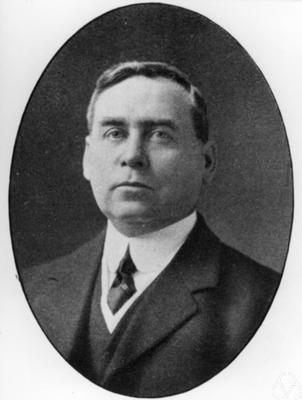
\includegraphics[width= 0.85\linewidth]{John_charles_fields}
		\caption{\small\textit{\color{lichsutoanhoc}Nhà toán học John Charles Fields. Nguồn: Wikipedia.}}
		\vspace*{-10pt}
	\end{figure}
	Phần lớn của bản ghi nhớ mang tính thủ tục: cách xử lý kinh phí, chỉ định một ủy ban, thông báo quyết định, thiết kế huy chương, v.v. Trên thực tế, Fields đã viết rằng ủy ban ``nên được càng tự do càng tốt" để quyết định người chiến thắng. Nhằm giảm thiểu sự ganh đua giữa các quốc gia, Fields quy định rằng huy chương không được đặt theo tên của bất kỳ cá nhân hay địa điểm nào, và không bao giờ có ý định đặt nó theo tên của chính mình. Lời chỉ dẫn nổi tiếng nhất của ông, sau này được sử dụng để giải thích cho giới hạn độ tuổi, là giải thưởng nên vừa là ``sự công nhận những việc đã làm được" vừa là ``sự khích lệ cho những thành tựu xa hơn nữa". Nhưng trong hoàn cảnh thời bấy giờ, chỉ dẫn này có một mục đích khác: ``để tránh những so sánh ngầm" giữa các nhóm theo chủ nghĩa dân tộc về việc ai xứng đáng giành chiến thắng. 
	\vskip 0.1cm
	Những huy chương đầu tiên được trao vào năm $1936$ cho hai nhà toán học Lars Ahlfors của Phần Lan và Jesse Douglas của Hoa Kỳ. Chiến tranh thế giới thứ hai đã làm trì hoãn các huy chương tiếp theo cho đến năm $1950$. Kể từ đó đến nay chúng được trao đều đặn bốn năm một lần.
	\vskip 0.1cm
	\textbf{\color{lichsutoanhoc}Máu và nước mắt}
	\vskip 0.1cm
	Quy trình lựa chọn huy chương Fields cần được giữ bí mật, nhưng các nhà toán học cũng là con người. Họ nói chuyện phiếm và đôi khi -- thật may mắn cho các nhà sử học -- lơ là trong việc bảo vệ những tài liệu mật, đặc biệt là trong những năm đầu của huy chương Fields, trước khi Liên đoàn toán học thế giới (International Mathematical Union--IMU) chính thức tham gia vào quá trình lựa chọn. Những phù du (ephemera) như vậy có lẽ là những tài liệu duy nhất còn sót lại.
	\vskip 0.1cm
	Ahlfors, một trong những nhà toán học được trao giải năm $1936$, đã phục vụ trong ủy ban lựa chọn huy chương Fields năm $1950$. Bản sao những thư từ trao đổi của ủy ban được chuyển thành một khối tài liệu liên quan đến ICM năm $1950$, phần lớn được lưu trữ tại Khoa Toán của Ahlfors tại Đại học Harvard (Cambridge, bang Massachusetts); những tài liệu này hiện vẫn đang nằm trong kho lưu trữ của đại học này.
	\vskip 0.1cm
	Ủy ban huy chương Fields năm $1950$ đến từ nhiều quốc gia. Chủ tịch của ủy ban là Harald Bohr (em trai của nhà vật lý Niels Bohr) đến từ Copenhagen (Đan Mạch). Các thành viên còn lại gồm Karol Borsuk (Warsaw, Ba Lan), Maurice Fréchet (Paris, Pháp), William Hodge (Cambridge, Anh), Damodar Kosambi (Tata, Ấn Độ) và Marston Morse (Princeton, Hoa Kỳ).\footnote[6]{\color{lichsutoanhoc}Nhà toán học Xô Viết Andrey Kolmogoroff được mời nhưng đã không tham gia ủy ban.}
	Họ liên lạc yếu thông qua các bức thư gửi cho Bohr, người sẽ tóm tắt những điểm chính trong các bức thư đó và gửi lại. Ủy ban đã tiến hành hầu hết các cuộc trao đổi này vào nửa cuối năm $1949$ và thống nhất về hai người chiến thắng vào tháng $12$ năm đó. 
	\vskip 0.1cm
	Các bức thư chỉ ra rằng Bohr đã tham gia vào quá trình tuyển chọn với một quan điểm mạnh mẽ về việc ai nên giành được một trong những huy chương: đó là nhà toán học người Pháp Laurent Schwartz, người đã gây ấn tượng mạnh với Bohr bằng một lý thuyết mới đầy thú vị tại một hội nghị vào năm $1947$ [$6$]. Chiến tranh thế giới thứ hai đồng nghĩa với việc sự nghiệp của Schwartz đã có một khởi đầu đặc biệt khó khăn: là một người Do Thái theo chủ nghĩa Trotsky\footnote[7]{\color{lichsutoanhoc}Hệ tư tưởng chính trị được phát triển và kế thừa từ chủ nghĩa Marx.} sống dưới chế độ Vichy của Pháp\footnote[8]{\color{lichsutoanhoc}Chính phủ Phát xít Pháp $(10.07.1940 - 09.08.1944)$.}, ông đã phải ẩn náu và dùng một cái tên giả che giấu thân phận. Cuốn sách chuyên khảo được chờ đợi từ lâu của ông cho đến cuối năm $1949$ vẫn chưa được xuất bản, cũng như có ít kết quả mới quan trọng được công bố.
	\vskip 0.1cm
	Bohr nhìn thấy ở Schwartz hình ảnh một nhà lãnh đạo toán học đầy lôi cuốn, người có thể đưa ra những cây cầu mới kết nối các lĩnh vực thuần túy và ứng dụng. Lý thuyết của Schwartz không hoàn toàn có được những tác động mang tính cách mạng như Bohr dự đoán, nhưng bằng cách quảng bá nó với huy chương Fields, Bohr đã thực hiện một sự can thiệp manh tính quyết định tới tương lai của Toán học.
	\vskip 0.1cm
	Bohr xác định cách tốt nhất để đảm bảo chiến thắng cho Schwartz là liên minh với Marston Morse của Viện Nghiên cứu Cao cấp Princeton, người về phần mình đang ủng hộ đồng nghiệp người Na Uy Atle Selberg. Con đường thuyết phục những thành viên còn lại của ủy ban không hề đơn giản, và các cuộc tranh luận của họ tiết lộ rất nhiều về suy nghĩ của các thành viên về huy chương Fields.
	\vskip 0.1cm
	Các thành viên ủy ban bắt đầu bằng việc thảo luận về các tiêu chí như tuổi và lĩnh vực nghiên cứu, thậm chí trước khi đề xuất những ứng viên. Hầu hết nghĩ rằng việc tập trung vào các nhánh cụ thể của toán học là không thể tránh khỏi. Họ đưa ra một loạt các cân nhắc về độ tuổi tiềm năng, chẳng hạn dưới $30$, cho đến một nguyên tắc chung rằng những người được đề cử nên đạt được thành tựu toán học trong khoảng thời gian từ ICM $1936$ cho đến thời điểm bấy giờ. Bohr đã gợi ý một cách khó hiểu rằng $42$ tuổi ``sẽ là một giới hạn tự nhiên của tuổi tác".
	\begin{figure}[H]
		\vspace*{-5pt}
		\centering
		\captionsetup{labelformat= empty, justification=centering}
		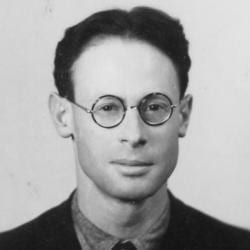
\includegraphics[width= 0.85\linewidth]{AndreWeil}
		\caption{\small\textit{\color{lichsutoanhoc}Đề cử nhà toán học Pháp André Weil đã chia rẽ ủy ban huy chương Fields năm 1950. Nguồn: buscabiografias.com.}}
		\vspace*{-10pt}
	\end{figure}
	Vào thời điểm danh sách đề cử đầu tiên lộ diện, gợi ý của Bohr trở nên sáng tỏ hơn rất nhiều. Rõ ràng mối đe dọa hàng đầu đối với các kế hoạch của ông dành cho Schwartz là một nhà toán học người Pháp khác, André Weil, người bước sang tuổi $43$ vào tháng $5$ năm $1949$. Tất cả mọi người, kể cả Bohr và Morse, đều đồng ý rằng Weil là nhà toán học xuất sắc hơn. Nhưng Bohr đã sử dụng yếu tố về tuổi tác để đảm bảo rằng Weil sẽ không giành chiến thắng. Với tư cách là chủ tịch, Bohr có một số quyền kiểm soát đối với các trao đổi và thường ám chỉ quan điểm lên các thành viên rằng các nhà toán học ``trẻ" nên được ưu tiên trong khi xem Schwartz là ví dụ điển hình của tuổi trẻ. Ông khẳng định rằng Weil đã ``quá nổi tiếng" và thu hút sự chú ý của mọi người vào lập luận của Ahlfors rằng việc trao huy chương cho Weil ``có thể là thảm họa" bởi vì ``nó sẽ tạo ấn tượng rằng ủy ban đã cố gắng chọn ra một thiên tài toán học vĩ đại nhất".
	\vskip 0.05cm
	Mục tiêu chính của ủy ban là tránh xung đột quốc tế và những so sánh tiềm ẩn. Nếu họ có thể phủ nhận việc đã cố gắng chọn ra những người xuất sắc nhất thì họ không thể bị buộc tội là đã bỏ qua ai đó tốt hơn.
	\vskip 0.05cm
	Tuy nhiên, Weil vẫn là một vấn đề. Ủy viên Damodar Kosambi nghĩ rằng sẽ là ``vô lý" nếu từ chối trao huy chương cho Weil -- một bình luận mà Bohr đã kể lại với một đồng nghiệp Đan Mạch nhưng không chia sẻ với các thành viên ủy ban khác. Ủy viên William Hodge lo lắng ``liệu chúng ta có thể trốn tránh trách nhiệm của mình hay không" nếu Weil không chiến thắng. Thậm chí Ahlfors còn cho rằng họ nên mở rộng giải thưởng cho bốn người để có thể bao gồm Weil. Bohr đã viết lại một lần nữa cho người đồng nghiệp Đan Mạch của mình rằng ``cần có nỗ lực phi thường" (blood and tears) để đem đến chiến thắng cho Schwartz và Selberg.
	\vskip 0.05cm
	Bohr thắng thế bằng cách cắt ngắn cuộc tranh luận. Ông lập luận rằng một chiến thắng cho Weil sẽ mở ra một cánh cửa để xem xét các nhà toán học cây đa cây đề, và yêu cầu ủy ban bỏ phiếu thuận hoặc chống đối với cặp Schwartz và Selberg. Cuối cùng, tại lễ trao giải ICM năm $1950$, Bohr ca ngợi Schwartz vì đã truyền cảm hững cho thế hệ các nhà toán học trẻ hơn -- điều ông cho rằng Weil không làm được.\footnote[9]{\color{lichsutoanhoc}Bohr đã dẫn trong thư gửi ủy ban: ``Anh ấy [Weil] là kiểu người luôn chỉ trích môi trường xung quanh dù anh ấy ở đâu".}
	\vskip 0.05cm
	\textbf{\color{lichsutoanhoc}Những khích lệ thêm}
	\vskip 0.05cm
	Những hồ sơ từ kho lưu trữ của Harvard cho thấy những cân nhắc vào năm $1950$ phản ánh những cái nhìn rộng hơn đối với huy chương Fields của các thành viên chứ không chỉ đơn thuần là của một vị chủ tịch nhiệt thành. Nhà toán học Harvard Oscar Zariski cũng lưu giữ các bức thư từ nhiệm kỳ của ông tại ủy ban năm $1958$ trong bộ sưu tập cá nhân.
	\vskip 0.05cm
	Ủy ban của Zariski do nhà toán học Heinz Hopf thuộc Viện Công nghệ Liên bang Thụy Sĩ ở Zurich (ETH Zürich) chủ trì. Vòng đề cử sơ bộ đã chọn ra đươc $38$ cái tên. Friedrich Hirzebruch là người có lợi thế rõ ràng và được đề cử bởi $5$ ủy viên.
	\vskip 0.05cm
	Hopf bắt đầu bằng việc gạch tên hai ứng viên lớn tuổi nhất là Lars Gårding và Lipman Bers. Động thái tiếp theo của ông đã chứng minh rằng không phải tuổi tác, mà sự công nhận trước mới thực sự là yếu tố bị loại: Hopf đã loại Hirzebruch và một người nữa, những người gần đây đã nhận được ghế giáo sư tại các học viện danh tiếng, bởi họ ``không cần khuyến khích thêm". Không ai trong ủy ban phản ứng dù chỉ là một chút.
	\vskip 0.05cm
	Trong số những người còn lại, ủy ban đồng ý rằng Alexander Grothendieck là người tài năng nhất, nhưng lại có ít kết quả đã được công bố. Vì vậy họ xem ông là ứng viên tiềm năng nhất cho $4$ năm sau ($1962$). John Nash, sinh cùng năm với Grothendieck ($1928$), đứng thứ ba trong vòng bỏ phiếu cuối cùng. Mặc dù danh sách rút gọn năm $1958$ có Olga Ladyzhenskaya và Harish--Chandra, nhưng phải đến năm $2014$ huy chương Fields mới thuộc về một phụ nữ (Maryam Mirzakhani)\footnote[10]{\color{lichsutoanhoc}Tại lễ trao giải $2022$ cách đây ít ngày, Maryna Viazovska đã trở thành nhà toán học nữ thứ hai giành huy chương Fields.} hoặc một nhà toán học gốc Ấn Độ (Manjul Bhargava)\footnote[11]{\color{lichsutoanhoc}Năm $2018$, Akshay Venkatesh là nhà toán học gốc Ấn Độ thứ hai được vinh danh.}. Cuối cùng, giải thưởng năm $1958$ đã được trao cho Klaus Roth và René Thom. Cả hai đều được ủy ban đánh giá là đầy hứa hẹn nhưng chưa quá thành công -- bởi vậy ít có khả năng gây ra những so sánh ngầm.
	\begin{figure}[H]
		\vspace*{-5pt}
		\centering
		\captionsetup{labelformat= empty, justification=centering}
		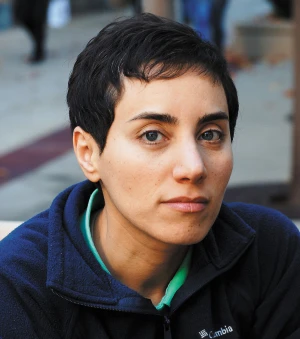
\includegraphics[width= 0.85\linewidth]{MaryamMirzakhani}
		\caption{\small\textit{\color{lichsutoanhoc}Maryam Mirzakhani, nhà toán học nữ đầu tiên được trao huy chương Fields. Nguồn: MaryamMirzakhani.}}
		\vspace*{-10pt}
	\end{figure}
	\textbf{\color{lichsutoanhoc}Bước ngoặt đột ngột}
	\vskip 0.05cm
	Đến năm $1966$, tiêu chuẩn các nhà toán học trẻ giỏi nhưng không phải quá giỏi đã trở nên khó khăn để đánh giá. Năm đó, chủ tịch của ủy ban là Georges de Rham đã thông qua giới hạn độ tuổi $40$, con số làm tròn nhỏ nhất bao trùm tuổi của tất cả những người giành được Fields trước đó. 
	\vskip 0.05cm
	Vậy là đột nhiên các nhà toán học mà trước đây được coi là quá thành công giờ lại đủ tiêu chuẩn. Grothendieck, người có lẽ bị loại vào năm $1962$ vì đã quá nổi tiếng, được trao huy chương vào năm $1966$. Tuy nhiên ông đã từ chối nhận giải vì lý do chính trị.
	\vskip 0.05cm
	Trong danh sách chiến thắng năm $1966$ còn có một nhà toán học hoạt động chính trị khác là Stephen Smale.\footnote[12]{\color{lichsutoanhoc}$1966$ là năm đầu tiên có $4$ người được trao huy hương Fields. Danh sách đầy đủ: Michael Atiyah, Paul Cohen, Alexander Grothendieck và Stephen Smale.}
	Ông đã đến Moscow nhận huy chương thay vì đứng điều trần trước Ủy ban Hạ viện Kiểm tra Hành động chống Hoa Kỳ (The US House Un--American Activities Committee) về hoạt động phản đối Chiến tranh Việt Nam của mình. Những nỗ lực của các đồng nghiệp để bảo vệ hành động này thu hút các hãng truyền thông lớn, và biệt danh ``giải Nobel toán học" cũng được ra đời từ đó.
	\vskip 0.05cm
	Sự trùng hợp ngẫu nhiên này -- so sánh huy chương Fields với một giải thưởng danh tiếng hơn đồng thời thay đổi quy tắc cho phép những người đã thành danh đạt huy chương -- đã có tác động lâu dài lên toán học cũng như lên hình ảnh của giải thưởng trong mắt công chúng. Nó đã viết lại hoàn toàn mục đích của huy chương, tách nó ra khỏi mục tiêu ban đầu là hòa giải quốc tế và dựa trên đúng những tiêu chuẩn mà Fields nghĩ sẽ chỉ làm gia tăng sự ganh đua.
	\begin{figure}[H]
		\vspace*{-5pt}
		\centering
		\captionsetup{labelformat= empty, justification=centering}
		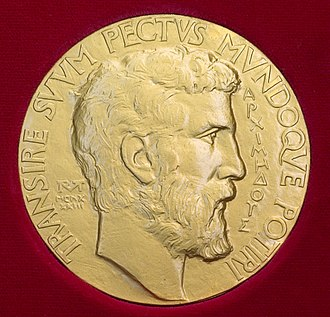
\includegraphics[width= 0.85\linewidth]{FieldsMedalFront}
		\caption{\small\textit{\color{lichsutoanhoc}Mặt trước huy chương Fields. Nguồn: Wikipedia.}}
		\vspace*{-10pt}
	\end{figure}
	Bất kỳ phương pháp nào để chọn ra một số ít người được vinh danh từ một lĩnh vực rộng lớn như Toán học sẽ luôn có những thiếu sót và tranh cãi. 
	Tuy nhiên, hoàn cảnh mang tính thể chế và xã hội có ảnh hưởng lớn đến việc ai có cơ hội để tiến xa trong lĩnh vực này ở mọi giai đoạn, từ tiểu học đến khi đã trở thành giáo sư. Bản thân các ủy ban tuyển chọn cần phải đa dạng và phù hợp với những giá trị và vai trò phức tạp của toán học trong xã hội. 
	\vskip 0.05cm
	Tuy có những sai sót, các quy trình trước năm $1966$ đã buộc một ủy ban gồm các nhà toán học ưu tú phải suy nghĩ nghiêm túc về tương lai lĩnh vực nghiên cứu của mình. Các ủy ban đã sử dụng huy chương như một công cụ phân phối lại, để tạo động lực cho những người mà họ cảm thấy không có mọi lợi thế nhưng vẫn đang làm công việc quan trọng.
	\vskip 0.05cm
	Hiểu biết hiện tại của chúng ta về tác động xã hội của toán học cũng như các rào cản để đa dạng hóa nó hoàn toàn khác với các nhà toán học giữa thế kỷ $20$. Nếu các ủy ban ngày nay cũng được trao quyền quyết định như những gì xảy ra vào thời kỳ đầu, họ có thể tập trung vào những nhà toán học mà công trình và tên tuổi của họ chưa được ghi nhận xứng đáng trong giới tinh hoa của ngành. Nhờ đó, họ có thể thúc đẩy những lĩnh vực nghiên cứu dựa trên những điều tốt đẹp mà chúng sẽ đưa đến cho thế giới, chứ không phải chỉ chú trọng vào độ khó của những định lý chúng đưa ra.
	\vskip 0.05cm
	Theo quan điểm của tôi, lịch sử của huy chương Fields là lời mời gọi  các nhà toán học ngày nay suy nghĩ một cách sáng tạo về tương lai cũng như về những thông điệp mà họ muốn truyền tải thông qua giải thưởng danh tiếng nhất của mình.
	\vskip 0.05cm
	\textbf{\color{lichsutoanhoc}Tài liệu tham khảo}
	\vskip 0.05cm
	[$1$] Barany, M. J. Not. Am. Math. Soc. $62$, $15-20$ $(2015)$.
	\vskip 0.05cm
	[$2$] Stern, N. Soc. Stud. Sci. $8$, $127-140$ $(1978)$.
	\vskip 0.05cm
	[$3$] Hersh, R. and John--Steiner, V. Loving + Hating Mathematics: Challenging the Myths of Mathematical Life $251-272$ (Princeton Univ. Press, $2011$). 
	\vskip 0.05cm
	[$4$] Henrion, C. AWM Newsletter $25$ $(6)$, $12-16$ $(1995)$.
	\vskip 0.05cm
	[$5$] Riehm, E. M. and Hoffman, F. Turbulent Times in Mathematics: The Life of J.C. Fields and the History of the Fields Medal (American Mathematical Society \& Fields Institute, $2011$).
	\vskip 0.05cm
	[$6$] Barany, M. J, Paumier, A.--S. and Lützen, J. Hist. Math. $44$, $367-394$ $(2017)$
\end{multicols}
\newpage
\blfootnote{$^1$\color{lichsutoanhoc}Cộng tác viên Viện Toán học.}
\begingroup
\AddToShipoutPicture*{\put(48,565){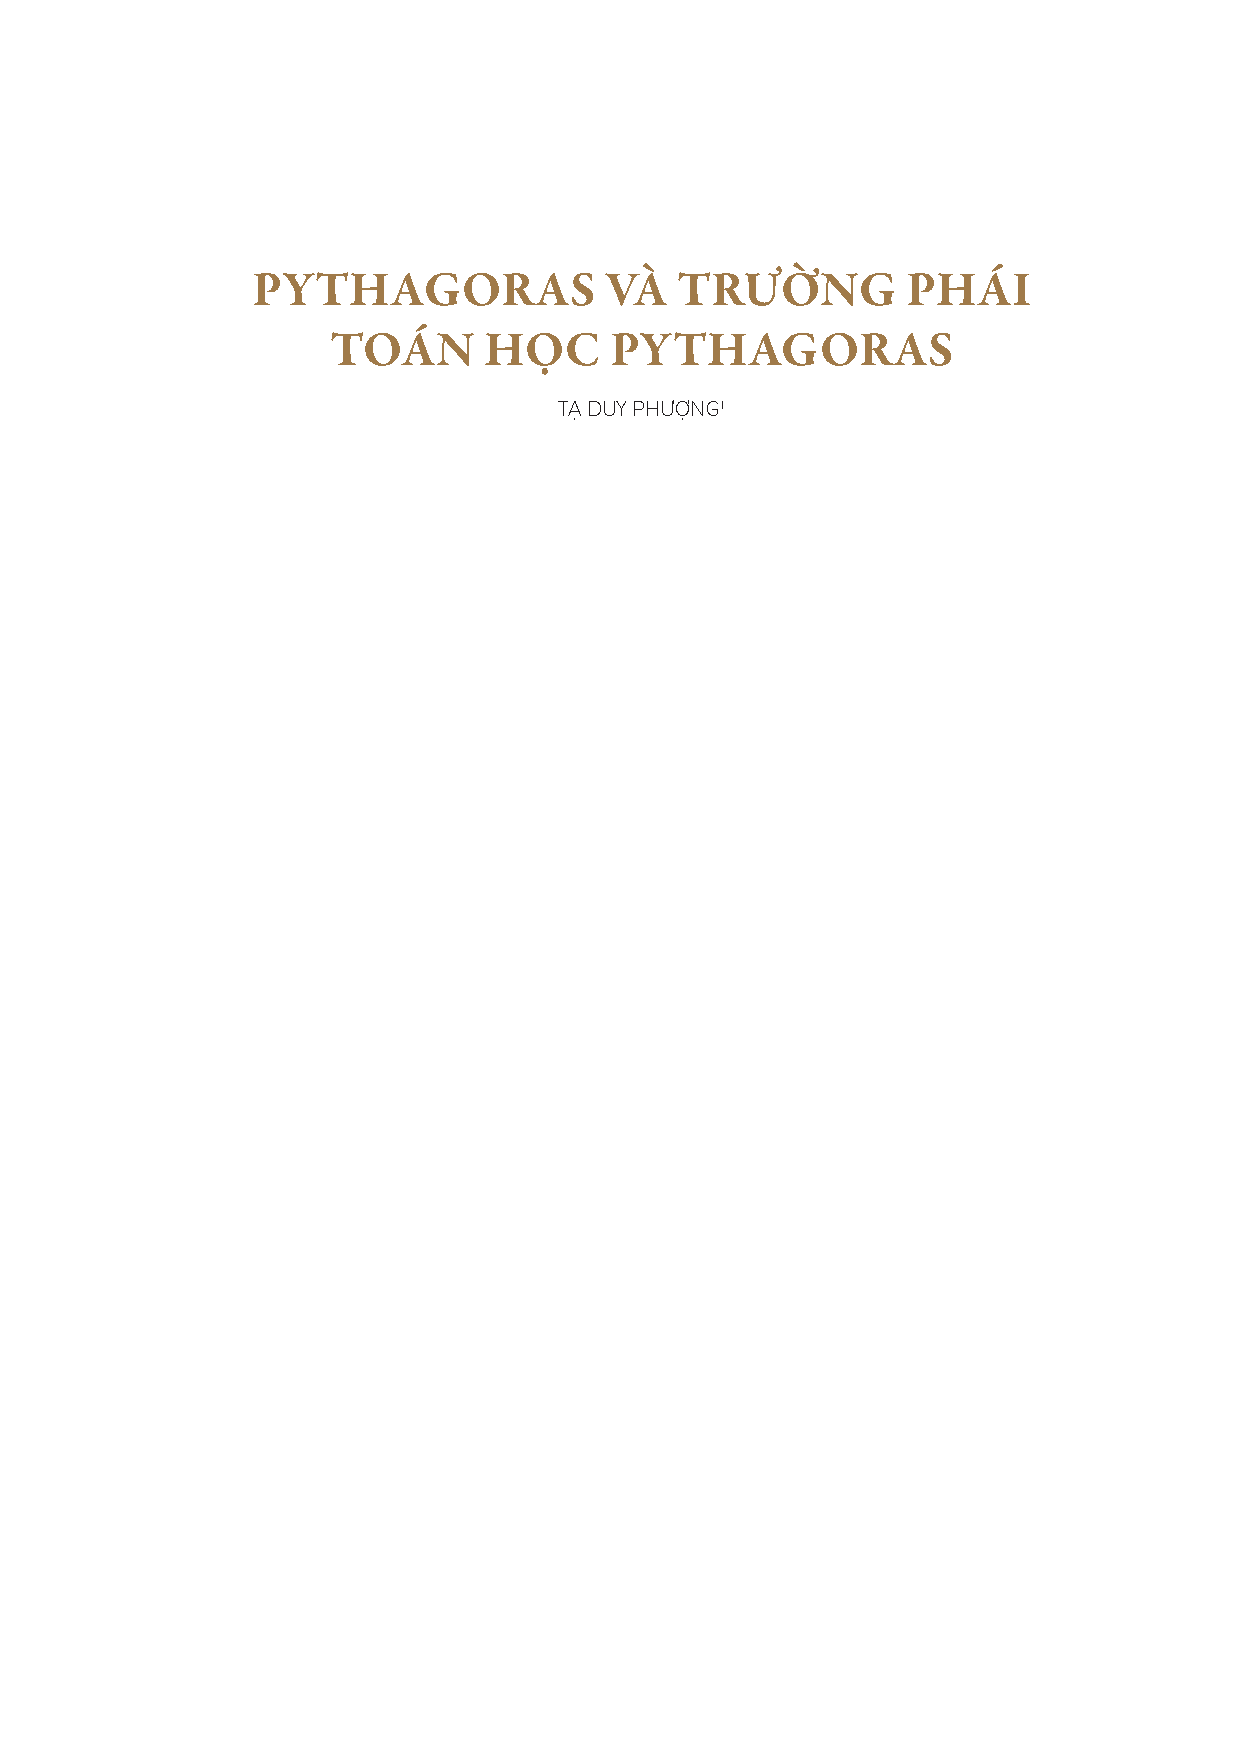
\includegraphics[scale=1]{../tieude.pdf}}}
\centering
\endgroup

\vspace*{145pt}

\begin{multicols}{2}
	\textbf{\color{lichsutoanhoc}Dẫn nhập}
	\vskip 0.1cm
	Nếu Thales (khoảng $625-547$ trước Công nguyên--TCN) và Pythagoras (khoảng $584-495$ TCN) là những người đặt nền móng cho sự phát triển một nghìn năm toán học Hy Lạp thì Euclid (khoảng $330-275$ TCN) và Archimedes (khoảng $330-275$ TCN) là những đỉnh cao của Toán học Hy Lạp nói riêng và Toán học nói chung. Trong bộ sách đồ sộ \textit{Elements (Cơ sở)}  gồm $13$ quyển, được dùng trong $2000$ năm, được tái bản nhiều lần với sửa chữa rất ít và sự phổ biến chỉ kém Kinh thánh, Euclid đã tiếp thu, hoàn thiện, hệ thống và phát triển toàn bộ kiến thức toán học thế giới đã đạt được trước đó, trong đó có thành tựu toán học Hy Lạp trong 300 năm từ thế kỷ V đến thế kỷ III trước Công nguyên. 
	\vskip 0.1cm
	Bài viết này giới thiệu những bài toán và kiến thức cơ bản đạt được bởi các nhà toán học Hy Lạp sau Pythagoras và trước Euclid. Ở một số chỗ, bài viết cũng liên hệ các thành tựu toán học thời kỳ này với Cơ sở của Euclid và toán học các thời kỳ sau.    
	\vskip 0.1cm
	\textbf{\color{lichsutoanhoc}Ba bài toán kinh điển: Cầu phương hình tròn, Bài toán chia ba một góc và Bài toán gấp đôi thể tích lập phương}
	\vskip 0.1cm
	Ba bài toán này đã thu hút các nhà toán học suốt $2000$ năm. Ở đây chúng ta thấy một toán học khác hoàn toàn với toán học Babilon và toán học Ai Cập. Đây không còn là ứng dụng thực tế của số học vào các vấn đề của đời sống, mà là sự phát triển toán học dựa trên nền tảng vững chắc  của suy luận, chứng tỏ sự khác biệt rõ ràng giữa các bài toán thực tế với phát triển tư duy và phát triển nội tại của toán học.
	\vskip 0.1cm
	\textbf{\color{lichsutoanhoc}Bài toán cầu phương hình tròn}
	\vskip 0.1cm
	Theo Plutarch ($46-119$ CN), trong thời gian ở trong tù, Anaxagoras (khoảng $500-428$ TCN) đã tìm cách giải bài toán cầu phương hình tròn, tức là bài toán dựng hình bằng thước và compass biến hình tròn thành hình vuông có cùng diện tích. 
	\vskip 0.1cm
	Nếu $r$ là bán kính hình tròn cho trước thì diện tích của nó bằng $\pi r^2$. Diện tích hình vuông cạnh $a$  là $a^2$. Suy ra  $a^2 = \pi r^2$ hay  $a=\sqrt{\pi}r$. Bài toán trở thành: Cho trước hai điểm $A,B$ Hãy dựng điểm $C$  trên đường thẳng  $AB$  sao cho $AC = \sqrt{r}AB$  hay $a= \sqrt{\pi}r$.
	\vskip 0.1cm 
	\textbf{\color{lichsutoanhoc}Bài toán gấp đôi thể tích hình lập phương}
	\vskip 0.1cm
	Anaxagoras mất vào năm $428$ TCN, đúng một năm trước khi Plato sinh ra và một năm sau nhà toán học Pericles mất. Tương truyền rằng Pericles chết vì bệnh dịch hạch, một bệnh dịch đã làm chết một phần tư dân số Athens, và thảm họa này đã là nguồn gốc cho bài toán toán học nổi tiếng thứ hai. Một phái đoàn Athens được cử đến nhà tiên tri của thần Apollo tại Delos để hỏi làm cách nào để ngăn chặn bệnh, và nhà tiên tri đã trả lời rằng bàn thờ hình khối lập phương cho thần Apollo phải được tăng gấp đôi về thể tích. Người Athens đã tăng gấp đôi kích thước của bàn thờ, nhưng bệnh dịch vẫn hoành hoành. Tất nhiên, bàn thờ đã được tăng gấp tám lần về thể tích, thay vì gấp hai lần như yêu cầu. Đây chính là bài toán: \textit{Dựng bằng thước và compass một cạnh của khối lập phương có thể tích gấp đôi khối đã cho.}
	\vskip 0.1cm
	Giả sử  $a$ là cạnh của lập phương đã cho,  $b$ là cạnh của lập phương cần tìm. Theo yêu cầu, ta có $b^3 = 2a^3$, tức là $b = \sqrt[3]{2}a$.  Bài toán trở thành: Cho hai điểm $A,B$. Tìm điểm  $C$ trên đường thẳng $AB$  sao cho $AC = \sqrt[3]{2}AB$  hay $b = \sqrt[3]{2}a$.
	\vskip 0.1cm 
	\textbf{\color{lichsutoanhoc}Bài toán chia ba một góc}
	\vskip 0.1cm
	Trong thời gian đó, lan truyền ở Athens một bài toán thứ ba cũng nổi tiếng không kém: Hãy dựng một góc bằng một phần ba góc đã cho nhờ thước kẻ và compass. Bài toán được phát biểu như sau: Cho hai điểm $A,B$ tùy ý trên đường tròn tâm $O$.  Tìm điểm $C$ trên cung $AB$ sao cho $\angle AOC = \dfrac{1}{3} \angle AOB$.
	\vskip 0.1cm  
	Ba bài toán: cầu phương hình tròn, gấp đôi cạnh của lập phương và bài toán chia ba một góc là ba bài toán nổi tiếng (ba bài toán kinh điển) của thời cổ đại. Để chứng minh cả ba bài toán này đều không giải được nếu chỉ dùng thước và compass, phải dùng đến lý thuyết trường đa thức . Điều này đã được các nhà toán học thế kỷ XIX (Lindemann,  Gauss, Wanzel, \ldots) giải quyết trọn vẹn.  
	\vskip 0.1cm
	\textbf{\color{lichsutoanhoc}Hippocrates: Bài toán cầu phương hình tròn  và Diện tích hình trăng khuyết}
	\vskip 0.1cm
	Nhà toán học lỗi lạc nhất Hy Lạp vào nửa sau thế kỷ V là Hippocrates xứ Chios. Ông sống vào khoảng $460-380$ TCN,  hơi trẻ hơn Anaxagoras. Cần phân biệt Ông  với bác sĩ nổi tiếng cùng tên và cùng thời Hippocrates xứ Cos (khoảng $460-370$ TCN). Giống như Thales, Hippocrates đã khởi nghiệp như một thương gia và trở thành nhà nghiên cứu toán học vào cuối đời. Aristotle cho rằng Hippocrates kém sắc sảo hơn Thales và do đó ông ta đã bị lừa hoặc bị cướp khi đi buôn. Hippocrates đã đến Athens để theo kiện. Phải ở lại Athens trong nhiều năm (vào khoảng những năm $430$ TCN), ông đã tham dự các bài giảng của một số triết gia. Có lý do để tin rằng những người Pythagoras (the Pythagoreans) đã định cư ở Athens vào thời điểm đó, vì vậy Ông có thể đã học họ mặc dù ông không có thầy chính thức là người Pythagoras. Cuối cùng, Hippocrates đã đạt được trình độ cao trong hình học đến mức ông trở thành một trong những người đầu tiên kiếm được tiền bằng dạy toán. Những người Pythagoras đã dạy Ông những gì họ biết về số học và hình học, sau đó Ông đã phản bội lòng tin của họ bằng cách bán những bí mật toán học của người Pythagoras cho bất kỳ ai mua (một cách giải thích nhẹ nhàng hơn là người Pythagoras, cảm thông với sự bất hạnh của Hippocrates, đã cho phép Ông kiếm tiền bằng cách dạy các kiến thức hình học của họ).
	\vskip 0.1cm
	Hippocrates coi thất bại trong kinh doanh là vận may của Ông, vì Ông đã có cơ hội tập trung nghiên cứu hình học, ở đó ông đã đạt được thành công đáng kể. 
	\vskip 0.1cm
	Vào giữa thế kỷ thứ V, rất nhiều định lý hình học đã được thiết lập dẫn tới sự cần thiết phải đưa tất cả kiến thức này vào một trật tự logic tốt. Proclus viết rằng Hippocrates đã viết cuốn  \textit{Cơ sở của hình học}, trước hơn một thế kỷ cuốn \textit{Cơ sở}  của Euclid. Tuy nhiên, cuốn sách của Hippocrates đã bị thất lạc, mặc dù nó đã được Aristotle ($384-322$ TCN) nói đến. Cuốn sách của Hippocrates có thể đã bắt đầu một truyền thống viết sách đáng chú ý, nhưng nó có những thiếu sót của một tác phẩm tiên phong, và do đó đã bị lỗi thời trước \textit{Cơ sở} của Euclid.
	\vskip 0.1cm
	Hippocrates đã trình bày hình học như một chuỗi các mệnh đề, một hình thức trình bày giống như cách trình bày hiện đại, trong đó các mệnh đề cần chứng minh có thể được suy ra trên cơ sở của những mệnh đề trước đó. Trong số những đổi mới khác, Ông đã sử dụng các chữ cái để ký hiệu các điểm và đường trong các hình hình học.
	\vskip 0.1cm
	Khi Hippocrates đến Athens, ba bài toán--cầu phương hình tròn, nhân đôi thể tích của khối lập phương và chia ba một góc--đã thu hút sự chú ý của các nhà hình học. Những bài toán này là các bài toán kinh điển trong lịch sử toán học, là  nguồn kích thích và say mê giống nhau cho những người nghiệp dư và học giả qua các thời đại, cho đến tận thế kỷ XIX và thậm chí cho tới thế kỷ XX, do không hiểu những bài toán này không thể giải được bằng thước và compass, nhiều nhà toán học nghiệp dư vẫn say sưa ``cầu phương hình tròn."
	\vskip 0.1cm
	Trong thực tế, không có tác phẩm toán học nào từ thế kỷ V TCN còn tồn tại, nhưng còn một chứng cớ là Simplicius (khoảng năm $520$ CN) tuyên bố đã sao chép theo nghĩa đen cuốn  \textit{Lịch sử Toán học} (đã mất) của Eudemus. Từ tuyên bố ngắn gọn này, chúng ta biết Hippocrates đã giải bài toán cầu phương hình trăng khuyết (hình giới hạn bởi hai cung tròn có bán kính không bằng nhau). Vấn đề cầu phương hình trăng khuyết chắc chắn đã nảy sinh từ bài toán cầu phương hình tròn và dựa trên khẳng định (của Hippocrates): \textit{Tỷ lệ diện tích các hình tròn có cùng tỷ lệ với các hình vuông nội tiếp các hình tròn ấy.}
	\vskip 0.1cm
	Ở đây Hippocrates đã sử dụng ngôn ngữ và khái niệm về tỷ lệ đóng một vai trò rất lớn trong tư tưởng của người Pythagoras. Trên thực tế, một số người cho rằng Hippocrates đã trở thành người theo trường phái Pythagoras. Trường Pythagoras ở Crotone đã bị đóng cửa, phái Pythagoras bị đàn áp (có thể vì tính bí mật, cũng có thể vì xu hướng chính trị bảo thủ của nó), nhưng sự phân tán của những người Pythagoras trên khắp thế giới tiếng Hy Lạp lại mở rộng ảnh hưởng của trường phái Pythagoras. Không nghi ngờ gì nữa, điều này đã ảnh hưởng, trực tiếp hoặc gián tiếp, tới Hippocrates.
	\vskip 0.1cm
	Trong mảnh sách còn lại của Eudemus có hai định lý sau (được coi là của Hippocrates). 
	\vskip 0.1cm
	\textbf{\color{lichsutoanhoc}Định lý} $\pmb{1.}$ Giả sử $AB$  là đường kính hình tròn tâm  $D$, $AC$  và $BC$  là hai cạnh của  hình vuông nội tiếp trong hình tròn ấy. Dựng nửa đường tròn $AEC$  đường kính  $AC$. Khi ấy diện tích hình trăng khuyết $AECFA$  bằng diện tích tam giác  $ADC$ (Hình $1a$).
	\begin{figure}[H]
		\vspace*{-5pt}
		\centering
		\captionsetup{labelformat= empty, justification=centering}
		\begin{tikzpicture}
			\draw [shift={(2.5,0.)},lichsutoanhoc]  plot[domain=0.:3.141592653589793,variable=\t]({1.*2.5*cos(\t r)+0.*2.5*sin(\t r)},{0.*2.5*cos(\t r)+1.*2.5*sin(\t r)});
			\draw [lichsutoanhoc] (0.,0.)-- (5.,0.);
			\draw [shift={(1.25,1.25)},lichsutoanhoc]  plot[domain=0.7853981633974483:3.9269908169872414,variable=\t]({1.*1.7677669529663689*cos(\t r)+0.*1.7677669529663689*sin(\t r)},{0.*1.7677669529663689*cos(\t r)+1.*1.7677669529663689*sin(\t r)});
			\draw [lichsutoanhoc] (2.5,2.5)-- (0.,0.);
			\draw [lichsutoanhoc] (2.5,2.5)-- (5.,0.);
			\draw [lichsutoanhoc] (2.5,2.5)-- (2.5,0.);
				\draw [fill=white] (0.,0.) circle (1.5pt);
				\draw[color=lichsutoanhoc] (-0.18,-0.19) node {$A$};
				\draw [fill=white] (5.,0.) circle (1.5pt);
				\draw[color=lichsutoanhoc] (5.16,-0.27) node {$B$};
				\draw[color=lichsutoanhoc] (1.12,2.47) node {$F$};
				\draw [fill=white] (2.5,0.) circle (1.5pt);
				\draw[color=lichsutoanhoc] (2.46,-0.23) node {$D$};
				\draw [fill=white] (2.5,2.5) circle (1.5pt);
				\draw[color=lichsutoanhoc] (2.64,2.83) node {$C$};
				\draw[color=lichsutoanhoc] (-0.12,2.89) node {$E$};
		\end{tikzpicture}
		\caption{\small\textit{\color{lichsutoanhoc}Hình $1a$.}}
		\vspace*{-10pt}
	\end{figure}
	\textit{Chứng minh}. Nối $C$ với $S$. Ký hiệu, thí dụ, ${S_{\bigcirc ACB}}$  là diện tích nửa hình tròn $ACB$ đường kính $AB$. Vì $AB^2 = 2AC^2$  (Hình $1a$)  nên 
	\begin{align*}
		\frac{{{S_{\bigcirc ACB}}}}{{{S_{\bigcirc AEC}}}} = \frac{{\pi {{\left( {\frac{{AB}}{2}} \right)}^2}}}{{\pi {{\left( {\frac{{AC}}{2}} \right)}^2}}} = \frac{{A{B^2}}}{{A{C^2}}} = 2
	\end{align*}
	hay ${S_{\bigcirc ACB}} = 2{S_{\bigcirc AEC}}.$
	\vskip 0.1cm
	Nhưng  ${S_{\bigcirc ACB}} = {S_{\bigcirc ADC}} + {S_{\bigcirc BDC}} = 2{S_{\bigcirc ADC}}$ nên ${S_{\bigcirc AEB}} = {S_{\bigcirc ADC}}$.   Suy ra 
	\begin{align*}
		{S_{AECFA}} + {S_{AFC}} = {S_{AECA}} = {S_{AFCA}} + {S_{\Delta ADC}}.
	\end{align*}
	Vậy diện tích hình trăng khuyết $AECFA$  bằng diện tích tam giác $ADC$,  hay trăng khuyết $AECFA$  đã được ``cầu phương".
	\vskip 0.1cm
	Một phiên bản khác của Định lý $1$ là
	\vskip 0.1cm
	\textbf{\color{lichsutoanhoc}Định lý} $\pmb{1'.}$ Dựng trên các cạnh của tam giác $ABC$ vuông ở $C$   các nửa đường tròn  đường kính $AB, AC, BC$. Khi ấy tổng diện tích hình trăng khuyết $L_1$  và $L_2$ bằng diện tích tam giác  $ABC$ (Hình $1b$).   
	\begin{figure}[H]
%		\vspace*{-5pt}
		\centering
		\captionsetup{labelformat= empty, justification=centering}
		\begin{tikzpicture}[scale=0.8]
			\draw [shift={(2.5,0.)},lichsutoanhoc]  plot[domain=0.:3.141592653589793,variable=\t]({1.*2.5*cos(\t r)+0.*2.5*sin(\t r)},{0.*2.5*cos(\t r)+1.*2.5*sin(\t r)});
			\draw [lichsutoanhoc] (0.,0.)-- (5.,0.);
			\draw [lichsutoanhoc] (3.390811455834727,2.33590559529995)-- (0.,0.);
			\draw [lichsutoanhoc] (3.390811455834727,2.33590559529995)-- (5.,0.);
			\draw [shift={(1.6954057279173635,1.167952797649975)},lichsutoanhoc]  plot[domain=0.6032325047411791:3.744825158330972,variable=\t]({1.*2.058765241544895*cos(\t r)+0.*2.058765241544895*sin(\t r)},{0.*2.058765241544895*cos(\t r)+1.*2.058765241544895*sin(\t r)});
			\draw [shift={(4.195405727917364,1.167952797649975)},lichsutoanhoc]  plot[domain=-0.9675638220537177:2.1740288315360754,variable=\t]({1.*1.418268550101352*cos(\t r)+0.*1.418268550101352*sin(\t r)},{0.*1.418268550101352*cos(\t r)+1.*1.418268550101352*sin(\t r)});
			\draw [shift={(2.5,0.)},lichsutoanhoc]  plot[domain=-3.141592653589793:0.,variable=\t]({1.*2.5*cos(\t r)+0.*2.5*sin(\t r)},{0.*2.5*cos(\t r)+1.*2.5*sin(\t r)});
				\draw [fill=white] (0.,0.) circle (1.5pt);
				\draw[color=lichsutoanhoc] (-0.26,-0.13) node {$A$};
				\draw [fill=white] (5.,0.) circle (1.5pt);
				\draw[color=lichsutoanhoc] (5.16,-0.27) node {$B$};
				\draw[color=lichsutoanhoc] (2.56,-0.15) node {$c$};
				\draw [fill=white] (3.390811455834727,2.33590559529995) circle (1.5pt);
				\draw[color=lichsutoanhoc] (3.54,2.71) node {$C$};
				\draw[color=lichsutoanhoc] (2.24,1.19) node {$b$};
				\draw[color=lichsutoanhoc] (3.78,1.45) node {$a$};
				\draw [fill=white] (1.6954057279173635,1.167952797649975) circle (1.5pt);
				\draw[color=lichsutoanhoc] (1.53,1.62) node {$S_1$};
				\draw [fill=white] (4.195405727917364,1.167952797649975) circle (1.5pt);
				\draw[color=lichsutoanhoc] (4.21,1.68) node {$S_2$};
				\draw[color=lichsutoanhoc] (0.75,2.86) node {$L_1$};
				\draw[color=lichsutoanhoc] (5.17,2.) node {$L_2$};
		\end{tikzpicture}
		\caption{\small\textit{\color{lichsutoanhoc}Hình $1b$.}}
		\vspace*{-10pt}
	\end{figure}
	\textit{Chứng minh}. Ta có   
	\begin{align*}
			{S_{\bigcirc AC}} + {S_{\bigcirc BC}} &= \pi {\left( {\frac{{AC}}{2}} \right)^2} + \pi {\left( {\frac{{BC}}{2}} \right)^2}\\
			&= \frac{\pi }{4}\left( {A{C^2} + B{C^2}} \right) \\
			&= \frac{\pi }{4}A{B^2} = {S_{\bigcirc ABC}}.
	\end{align*}
	Hay (Hình $1b$)
	\begin{align*}
		{S_{{L_1}}} + {S_{{S_1}}} + {S_{{L_2}}} + {S_{{S_2}}} = {S_{\Delta ABC}} + {S_{{S_1}}} + {S_{{S_2}}}.
	\end{align*}
	Suy ra
	\begin{align*}
		{S_{{L_1}}} + {S_{{L_2}}} = {S_{\Delta ABC}}.
	\end{align*}
	\textbf{\color{lichsutoanhoc}Định lý} $\pmb{2}.$ Diện tích nửa lục giác đều $CEFD$ bằng tổng diện tích nửa hình tròn $ALB$  và ba hình trăng khuyết $CGEMC$,  $EHFNE$, $FKDOF$ (Hình $2$).
	\begin{figure}[H]
		\vspace*{-10pt}
		\centering
		\captionsetup{labelformat= empty, justification=centering}
		\begin{tikzpicture}[scale=0.8]
			\draw [lichsutoanhoc] (-5.,0.)-- (-3.,0.);
			\draw [shift={(-4.,0.)},lichsutoanhoc]  plot[domain=0.:3.141592653589793,variable=\t]({1.*1.*cos(\t r)+0.*1.*sin(\t r)},{0.*1.*cos(\t r)+1.*1.*sin(\t r)});
			
			\draw [fill=white] (-5.,0.) circle (1.5pt);
			\draw[color=lichsutoanhoc] (-4.86,0.37) node {$A$};
			\draw [fill=white] (-3.,0.) circle (1.5pt);
			\draw[color=lichsutoanhoc] (-2.86,0.37) node {$B$};
			
			\draw[color=lichsutoanhoc] (-3.82,1.29) node {$L$};
		\end{tikzpicture}
		\caption{\small\textit{\color{lichsutoanhoc}Hình $2a$.}}
		\vspace*{-10pt}
	\end{figure}
	\begin{figure}[H]
		\vspace*{-10pt}
		\centering
		\captionsetup{labelformat= empty, justification=centering}
		\begin{tikzpicture}[scale=0.8]
			\draw [lichsutoanhoc] (-1.,0.)-- (5.,0.);
			\draw [shift={(2.,0.)},lichsutoanhoc]  plot[domain=0.:3.141592653589793,variable=\t]({1.*3.*cos(\t r)+0.*3.*sin(\t r)},{0.*3.*cos(\t r)+1.*3.*sin(\t r)});
			\draw [shift={(-0.25,1.299038105676658)},lichsutoanhoc]  plot[domain=1.0471975511965979:4.188790204786391,variable=\t]({1.*1.5*cos(\t r)+0.*1.5*sin(\t r)},{0.*1.5*cos(\t r)+1.*1.5*sin(\t r)});
			\draw [shift={(2.,2.598076211353316)},lichsutoanhoc]  plot[domain=0.:3.141592653589793,variable=\t]({1.*1.5*cos(\t r)+0.*1.5*sin(\t r)},{0.*1.5*cos(\t r)+1.*1.5*sin(\t r)});
			\draw [shift={(4.25,1.299038105676658)},lichsutoanhoc]  plot[domain=-1.0471975511965983:2.0943951023931953,variable=\t]({1.*1.5*cos(\t r)+0.*1.5*sin(\t r)},{0.*1.5*cos(\t r)+1.*1.5*sin(\t r)});
			\draw [lichsutoanhoc] (-1.,0.)-- (0.5,2.598076211353316);
			\draw [lichsutoanhoc] (0.5,2.598076211353316)-- (3.5,2.598076211353316);
			\draw [lichsutoanhoc] (3.5,2.598076211353316)-- (5.,0.);
		
				\draw [fill=white] (-1.,0.) circle (1.5pt);
				\draw[color=lichsutoanhoc] (-1.08,-0.33) node {$C$};
				\draw [fill=white] (5.,0.) circle (1.5pt);
				\draw[color=lichsutoanhoc] (5.2,-0.29) node {$D$};
				\draw [fill=white] (0.5,2.598076211353316) circle (1.5pt);
				\draw[color=lichsutoanhoc] (0.6,2.31) node {$E$};
				\draw [fill=white] (3.5,2.598076211353316) circle (1.5pt);
				\draw[color=lichsutoanhoc] (3.32,2.33) node {$F$};
				\draw[color=lichsutoanhoc] (-1.72,2.39) node {$G$};
				\draw[color=lichsutoanhoc] (1.98,4.53) node {$H$};
				\draw[color=lichsutoanhoc] (5.72,2.35) node {$K$};
				\draw[color=lichsutoanhoc] (-0.84,1.87) node {$M$};
				\draw[color=lichsutoanhoc] (2.,3.43) node {$N$};
				\draw[color=lichsutoanhoc] (4.86,1.65) node {$O$};
		\end{tikzpicture}
		\caption{\small\textit{\color{lichsutoanhoc}Hình $2b$.}}
		\vspace*{-5pt}
	\end{figure}
	\textit{Chứng minh}. Dựng nửa hình tròn đường kính $AB = \dfrac{1}{2}CD$ (Hình $2a$). Dựng các nửa hình tròn đường kính $CE, EF, FD$ là ba cạnh liên tiếp của lục giác đều nội tiếp đường tròn đường kính  $CD$ (Hình $2b$). Vì 
	\begin{align*}
		C{D^2} = 4A{B^2} = A{B^2} + C{E^2} + E{F^2} + F{D^2}
	\end{align*}
	và tỷ lệ diện tích các hình tròn bằng tỷ lệ diện tích các hình vuông dựng trên đường kính của chúng nên 
	\begin{align*}
		&{S_{\bigcirc CEFD}} \\
		= &{S_{\bigcirc ALB}} + {S_{\bigcirc CGE}} + {S_{\bigcirc EHF}} + {S_{\bigcirc FKD}}.
	\end{align*}
	Trừ hai vế cho tổng diện tích ba hình viên phân $CMEC, ENFE, FODF$  ta được  
	\begin{align*}
		&{S_{CEFD}} \\
		= &{S_{\bigcirc ALB}} + {S_{CGEMC}} + {S_{EHFNE}} + {S_{FKDOF}}.
	\end{align*}
	Eudemus tin rằng Hippocrates đã chứng minh hai định lý trên, nhưng một chứng minh nghiêm túc vào thời điểm đó (khoảng năm $430$ trước Công nguyên) dường như khó có thể xảy ra. Chứng minh trong Quyển $12$ Chương $2$ \textit{Cơ sở} của Euclid dường như là của Eudoxus, một nhà toán học sống nửa thời gian giữa Hippocrates và Euclid. Tuy nhiên, hai cuốn sách đầu của Euclid dường như bắt nguồn từ Pythagoras, vì vậy sẽ có vẻ hợp lý khi giả định rằng công thức, ít nhất, phần lớn cuốn sách III và IV của \textit{Cơ sở}  là từ tác phẩm của Hippocrates. Hơn nữa, nếu Hippocrates đã đưa ra một chứng minh định lý về diện tích của các hình giới hạn bởi các hình tròn, thì Hippocrates chính là người phát minh ra phương pháp chứng minh gián tiếp trong toán học. 
	\vskip 0.1cm
	Từ các định lý về diện tích hình trăng khuyết, Hippocrates được coi là người đầu tiên trong lịch sử toán học tìm ra cách tính diện tích các hình cong (khác hình tròn). 
	\vskip 0.1cm
	Có cơ sở tương đối vững chắc về mặt lịch sử  khi nói rằng cầu phương hình tròn đã được phát triển bởi Hippocrates. Các học giả ngoài Simplicius cũng đề cập đến tác phẩm của Hippocrates. Simplicius sống ở thế kỷ VI, nhưng ông không chỉ trích dẫn Eudemus (khoảng năm $320$ TCN) mà còn dựa vào Alexander xứ Aphrodisias (khoảng năm $200$ CN), một trong những nhà bình luận chính về Aristotle. 
	Các kết quả trên dường như đã khuyến khích Hippocrates, cũng như những người cùng thời và những người kế nhiệm ông hi vọng rằng cuối cùng hình tròn sẽ được cầu phương.
	\vskip 0.1cm
	Các kết quả của Hippocrates về cầu phương hình trăng khuyết có thể coi là những nỗ lực đáng kể của toán học vào thời điểm đó. Nó cho thấy rằng các nhà toán học Athens rất thành thạo trong việc xử lý các phép biến đổi diện tích và tỷ lệ.
	\vskip 0.1cm 
	Có ba quan điểm về những gì Hippocrates đã suy luận từ cầu phương hình trăng khuyết. Một số đã buộc tội Ông vì tin rằng Ông có thể cầu phương tất cả các hình trăng, trong đó có hình tròn; Những người khác nghĩ rằng Ông biết những hạn chế công việc của mình, biết rằng nó được chứng minh chỉ với một số loại hình trăng. Một học giả lại viết rằng Hippocrates biết Ông đã không cầu phương hình tròn nhưng cố đánh lừa đồng hương là mình đã thành công. 
	\vskip 0.1cm
	Hippocrates còn là người đầu tiên sử dụng ký hiệu chữ cái trong các hình hình học. Thật thú vị khi lưu ý rằng trong khi Hippocrates có đóng góp trong hai bài toán nổi tiếng, Ông dường như đã không có tiến bộ trong bài toán chia ba một góc, một vấn đề được nghiên cứu phần nào sau đó bởi Hippias của Elis.
	\vskip 0.1cm
	\textbf{\color{lichsutoanhoc}Hippias xứ Elis}
	\vskip 0.1cm
	Vào cuối thế kỷ thứ năm TCN, một nhóm giáo viên chuyên nghiệp hoàn toàn không giống như người Pythagoras nổi lên mạnh mẽ ở Athens. Trong số này có Hippias, một người gốc Elis, đã sống tại Athens vào nửa sau của thế kỷ thứ năm TCN.  Ông là một trong những nhà toán học đầu tiên mà chúng ta có thông tin trực tiếp, vì chúng ta đọc được nhiều điều về Ông từ \textit{Đối thoại} của Plato. Ông được cho là đã viết nhiều, từ toán học để diễn xướng, nhưng không có tác phẩm nào của Ông còn tồn tại.  
	\vskip 0.1cm
	Hippias (khoảng $500-401$ TCN)  sống cùng thời với Socrates (khoảng $477-399$ TCN). Socrates được cho là đã mô tả Hippias đẹp trai, học giỏi nhưng khoe khoang và nông nổi. Trong \textit{Đối thoại} của Plato và \textit{Những kỷ vật} của Xenophon có những nhận xét không mấy hay ho về Hippias như một người tự coi mình là một chuyên gia trong mọi thứ từ lịch sử và văn học đến thủ công mỹ nghệ và khoa học. 
	\vskip 0.1cm
	Proclus và các nhà toán học khác đã gán tên trisectrix hoặc quadratrix cho Hippias, các đường cong khác đường tròn và đường thẳng. Điều này được mô tả như sau: Trong hình vuông $ABCD$ (Hình $3$), cho cạnh $AB$ di chuyển đều từ vị trí hiện tại của nó cho đến khi nó trùng với $DC$ và để chuyển động này diễn ra chính xác cùng thời gian $DA$ quay theo chiều kim đồng hồ từ vị trí hiện tại của nó cho đến khi nó trùng với $DC$.
	\begin{figure}[H]
		\vspace*{-5pt}
		\centering
		\captionsetup{labelformat= empty, justification=centering}
		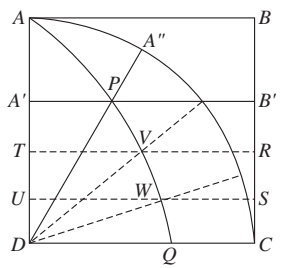
\includegraphics[width = 0.85\linewidth]{1}
		\caption{\small\textit{\color{lichsutoanhoc}Hình $3$.}}
		\vspace*{-10pt}
	\end{figure}
	Nếu vị trí của hai đường chuyển động tại bất kỳ thời gian tương ứng được cho bởi $AuBu$ và $DAv$, và nếu $P$ là điểm của giao điểm của $AuBu$ và $DAv$, quỹ tích của $P$ trong quá trình chuyển động sẽ là trisectrix của Hippias -- đường cong $APQ$ trong Hình $3$. Với đường cong này, việc cắt bỏ một góc được thực hiện một cách dễ dàng. Ví dụ: nếu $PDC$ là góc được cắt bỏ, người ta chỉ cần cắt các đoạn $BuC$ và $AuD$ tại các điểm $R$, $S$, $T$ và $U$. Nếu đường $TR$ và $US$ cắt trisectrix ở $V$ và $W$, tương ứng, các dòng $VD$ và $WD$, theo thuộc tính của trisectrix, chia góc $PDC$ thành ba phần bằng nhau. Đường cong Hippias thường được gọi là quadratrix, vì nó có thể được sử dụng để cầu phương hình tròn. Người ta đã phỏng đoán rằng Hippias biết về phương pháp cầu phương này nhưng cầu phương qua đường cong Hippias do Dinostratus đưa ra sau này.
	\vskip 0.1cm
	Về tính cách, Plato đối lập Hippias với Socrates, người ta có thể tạo ra nhiều sự tương phản giống nhau bằng cách so sánh Hippias với một người cùng thời khác--nhà toán học thuộc trường phái Pythagoras là Archytas xứ Tarentum.
	\vskip 0.1cm
	\textbf{\color{lichsutoanhoc}Philolaus và Archytas xứ Tarentum}
	\vskip 0.1cm  
	Pythagoras được cho là đã lui về Metapontum vào cuối đời và đã chết ở đó khoảng năm $500$ TCN.  Ông không để lại các tác phẩm viết, nhưng ý tưởng của Ông đã được thực hiện bởi một số lượng lớn đệ tử. Trung tâm ở Croton đã bị bỏ hoang khi một nhóm đối thủ chính trị từ Sybaris đã bất ngờ sát hại nhiều thủ lĩnh, nhưng những người thoát khỏi vụ thảm sát đã mang theo các học thuyết của trường phái Pythagoras đến các khu vực khác của thế giới Hy Lạp. Trong số những người học được từ những người tị nạn Pythagoras có Philolaus xứ Tarentum. Ông được cho là đã viết bài tường thuật đầu tiên về thuyết Pythagoras.  Rõ ràng, đây là cuốn sách mà từ đó Plato rút ra kiến thức của Ông về Pythagoras.  
	\vskip 0.1cm
	Sự cuồng tín số rất đặc trưng của Pythagoras hiển nhiên đã được chia sẻ bởi Philolaus. Ông giải thích phần lớn những truyền thuyết huyền bí cũng như kiến thức về vũ trụ học của Pythagoras. Các Sơ đồ vũ trụ của Philolaus được cho là đã được sửa đổi bởi hai người thuộc trường phái Pythagoras, Ecphantus và Hicetas, những người đã giải thích ngày và đêm bằng cách đặt trái đất quay.  
	\vskip 0.1cm
	Sự cực đoan của việc tôn thờ số của Philolaus dường như cũng đã trải qua một số sửa đổi, đặc biệt hơn là dưới bàn tay của Archytas, một học trò của Philolaus xứ Tarentum. 
	\vskip 0.1cm
	Archytas tin tưởng chắc chắn vào hiệu quả của số. Trong nhiều năm liên tiếp, ông được bầu làm tướng, và Ông chưa bao giờ bị đánh bại. Ông tốt bụng và là một người yêu trẻ em, vì Ông là được cho là đã phát minh ra ``rchytas's rattle", một đồ chơi bằng gỗ, được chế tạo để làm thú vui cho trẻ. Archytas tiếp tục truyền thống Pythagoras trong việc đặt số học lên trên hình học, nhưng sự nhiệt tình của Ông đối với con số nhẹ hơn ở Philolaus.  Ông đã viết ứng dụng của số học, hình học đối với âm nhạc, và có thể là Philolaus hoặc Archytas đã đưa ra khái niệm ``trung bình điều hòa". 
	\vskip 0.1cm
	Archytas đã chú ý nhiều đến âm nhạc nhiều hơn so với những người tiền nhiệm của mình và Ông cảm thấy rằng môn học này phải đóng một vai trò lớn hơn văn học trong việc giáo dục trẻ em. Archytas dường như đã chú ý đáng kể đến vai trò của toán học trong chương trình giảng dạy, và Ông được coi là đã chỉ định bốn nhánh trong tứ giác toán học -- số học (hoặc số còn lại), hình học (hoặc độ lớn khi dừng lại), âm nhạc (hoặc các con số đang chuyển động) và thiên văn học (hoặc độ lớn trong chuyển động). Các môn học này, cùng với bộ ba bao gồm ngữ pháp, tu từ và biện chứng (mà Aristotle bắt nguồn từ Zeno), sau này tạo thành bảy nghệ thuật tự do; vì thế Archytas được coi là có đóng góp nổi bật đưa vai trò của toán học lên một vị trí quan trọng trong giáo dục. 
	\vskip 0.1cm
	Tuy nhiên, đóng góp quan trọng nhất của Archytas cho toán học có thể là sự can thiệp của ông với bạo chúa Dionysius để cứu sống người bạn Plato của mình. Plato cho đến cuối cuộc đời vẫn cam kết sâu sắc với sự tôn kính Pythagoras về số và hình học, và vị thế tối cao của Athens trong thế giới toán học của thế kỷ thứ tư TCN là kết quả chủ yếu từ sự nhiệt tình của Plato, ``nhà tạo ra các nhà toán học." 
	\vskip 0.1cm
	\textbf{\color{lichsutoanhoc}Menaechmus}
	\vskip 0.1cm
	Eudoxus được ghi nhớ trong lịch sử toán học không chỉ vì công việc của riêng mình mà còn thông qua học sinh của mình. 
	\vskip 0.1cm
	Ở Hy Lạp, có một sợi dây tiếp nối truyền thống từ thầy sang trò.  Thí dụ, Plato học được từ Archytas, Theodorus và Theaetetus; ảnh hưởng của Plato lần lượt được truyền qua Eudoxus cho anh em Menaechmus và Dinostratus, cả hai đều đạt được thành tựu xuất sắc trong toán học. 
	\vskip 0.1cm
	Menaechmus nổi tiếng là người đã khám phá ra các đường cong mà sau này được gọi là hình elip, parabol và hyperbol, các thiết diện được cắt ra bởi hình nón (các đường cong conic).
	\vskip 0.1cm
	Menaechmus đã thành công dựa trên các đường cong conic với các tính chất thích hợp để giải bài toán gấp đôi khối lập phương. 
	\vskip 0.1cm
	Proclus đã viết rằng Menaechmus là một trong những người đã ``làm cho toàn bộ hình học trở lên hoàn hảo hơn" (made the whole of geometry more perfect). Chúng ta biết rằng Menaechmus đã dạy Alexander Đại đế, và huyền thoại nổi tiếng thuộc về Menaechmus, khi học trò của Ông yêu cầu một lối tắt đến hình học: ``Hỡi Vua, để đi qua đất nước, có những con đường hoàng gia và những con đường dành cho công dân chung; nhưng trong hình học, chỉ có một con đường cho tất cả mọi người". ``O King, for traveling over the
	country there are royal roads and roads for common citizens; but in geometry there is one road for all."
	\vskip 0.1cm 
	Chứng cứ Menaechmus phát hiện ra các thiết diện conic là do một lá thư từ Eratosthenes đến Vua Ptolemy Euergetes, được Eutocius trích dẫn khoảng $700$ năm sau đó, trong đó bài toán gấp đôi khối lập phương được đề cập. 
	\vskip 0.1cm
	\textbf{\color{lichsutoanhoc}Dinostratus và cầu phương hình tròn}
	\vskip 0.1cm
	Dinostratus, anh trai của Menaechmus, cũng là một nhà toán học; một người đã ``giải quyết" bài toán gấp đôi khối lập phương, người còn lại ``giải quyết" bài toán cầu phương hình tròn. 
	\vskip 0.1cm
	\textbf{\color{lichsutoanhoc}Thay lời kết}
	\vskip 0.1cm
	Tất nhiên, người Hy Lạp cũng hiểu rằng việc sử dụng đường cong trong các bài toán chia ba góc và các bài toán cầu phương đã vi phạm quy tắc của trò chơi—chỉ cho phép sử dụng compass và thước thẳng. ``Lời giải" của Hippias, Menaechmus và Dinostratus, như các tác giả của chúng cũng nhận ra, là ngụy tạo; vì thế, việc tìm kiếm các giải pháp khác, chính tắc hoặc bất hợp pháp, tiếp tục, với kết quả là một số đường cong mới đã được phát hiện bởi các nhà hình học Hy Lạp.
	\vskip 0.1cm
	\textbf{\color{lichsutoanhoc}Tài liệu tham khảo chính}
	\vskip 0.1cm
	[$1$] David M. Burton, \textit{The History of Mathematics, An Introduction, Seventh Edition}, McGraw--Hill, $2011$. Chapter $3$: The Beginnings of Greek Mathematics, $3.2$ Pythagorean Mathematics, pp. $116-139$.
	\vskip 0.1cm
	[$2$] Thomas Heath, \textit{A History of Greek Mathematics, Oxford at the Clarendon Press}, $1921$, Volume $1$: From Thales to Euclid, pp. $170-353$.
	\vskip 0.1cm   
	[$3$] Victor J. Katz, \textit{A History of Mathematics, An Introduction}, Third Edition, Addison--Wesley, $2009$. Chapter $2$: \textit{The Beginnings of Mathematics in Greek}, pp. $40-49$.
	\vskip 0.1cm
	[$4$] Uta C. Merzbach and Carl B. Boyer, \textit{A
	History of Mathematics}, Third Edition, John Wiley \& Sons, $2011$, trang $57-89$.
	\vskip 0.1cm
	[$5$] Ngô Việt Trung, \textit{Lý thuyết Galois về các vấn đề giải phương trình bằng căn thức, dựng hình bằng thước kẻ và compa}, Nhà xuất bản Đại học Quốc gia Hà Nội, $2006$.
	\vskip 0.1cm
	\textbf{\color{lichsutoanhoc}Tài liệu tham khảo}
	\vskip 0.1cm 
	[$6$] George Johston Allman, \textit{Greek Geometry: From Thales to Euclid}, Dublin Universty Press, $1877$, $432$ trang.  
	\vskip 0.1cm
	[$7$] Euclid, \textit{Cơ sở của Hình học}, Nhà xuất bản Trí thức, $2016$, $350$ trang.
	\vskip 0.1cm
	[$8$] R. Lloyd, \textit{Early Greek Science: Thales to Aristotle}, $1970$, Chatto \& Windus, London, $156$ trang. 
	\vskip 0.1cm
	[$8$] Nicomachus of Gerasa, \textit{Introduction to Arithmetic}, Translated into English by Martin Luther D’ooge, The Macmillan Company, New York, $1926$.
	\vskip 0.1cm
	[$9$] Proclus, \textit{Commentaries on Euclid’s books}, Vol. $1$, $330$ trang.
	\vskip 0.1cm
	[$10$] Arpad Szabo, \textit{The beginnings of Greek Mathematics}, Springer, $1978$, $363$ trang.
	\vskip 0.1cm
	[$11$] M. L. West, \textit{Early Greek Philosophy and the Orient}, Oxford at the Clarendon Press, $1971$, $255$ trang.
\end{multicols}
%\vspace*{-5pt}
%\rule{1\linewidth}{0.1pt}
%\begin{center}
%	\textbf{\LARGE\color{lichsutoanhoc}LỜI GIẢI, ĐÁP ÁN}
%\end{center}
%	
%\begin{multicols}{2}
%	\textbf{Bác nông dân tốt bụng}
%	\vskip 0.1cm
%	Do bác nông dân đi xuyên qua rừng với vận tốc bằng nửa so với vận tốc đi trên đường cái, nên trong hai ngày đêm (thứ hai và thứ ba) bác chỉ đi được quãng đường bằng quãng đường đi được trong cả ngày đêm thứ nhất, có nghĩa là một phần ba quãng đường. Vì thế $30$ km đi được trong ngày và đêm thứ tư cũng chính là $1/3$ quãng đường. Vậy bác nông dân đã đi hết $90$ km. Con đường đi của bác nông dân được biểu diễn bằng màu xanh như trên hình vẽ. 
%	\begin{figure}[H]
%		\vspace*{-5pt}
%		\centering
%		\captionsetup{labelformat= empty, justification=centering}
%		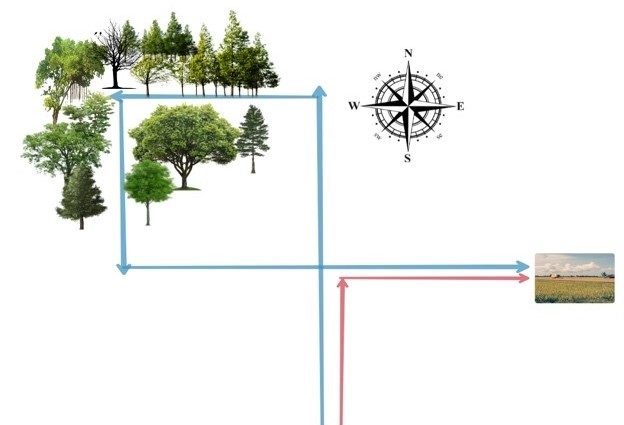
\includegraphics[width= 1\linewidth]{lgxp}
%		\vspace*{-10pt}
%	\end{figure}
%	Xuân Phong đã lập luận như sau: nếu chỉ đi nửa đoạn đường lên phía bắc rồi quay ngay sang hướng đông, thì chỉ hết nửa ngày nữa là thám tử đã đến Vườn Ngô, sau khi đi nửa quãng đường về phía bắc và nửa quãng đường về phía đông, có nghĩa là thám tử chỉ cần đi có $30$ km (theo con đường màu đỏ). 
%	\vskip 0.1cm
%	\textbf{Đố vui}
%	\vskip 0.1cm 
%	Có thể dễ dàng chỉ ra rằng với hai chiếc máy bay, Gru không thể thực hiện được kế hoạch của mình. Với ba chiếc máy bay thì Gru có thể thực hiện được, chẳng hạn với chiến lược sau đây.
%	\vskip 0.1cm   
%	Đầu tiên, ba máy bay, một chiếc của Gru và hai chiếc khác để hỗ trợ Gru, cùng xuất phát từ sân bay. Sau khi đi được $1/8$ vòng Trái Đất, một máy bay tiếp nhiên liệu cho cả máy bay của Gru và chiếc còn lại, mỗi chiếc $1/4$ bình (nếu coi mỗi chiếc máy bay có $1$ bình nhiên liệu) và giữ lại cho mình $1/4$ bình. Khi này, hai chiếc máy bay có đầy bình và một chiếc có $1/2$ bình (vừa đủ để có thể quay lại sân bay ban đầu).  Sau đó, hai máy bay có đầy bình tiếp tục hành trình của mình còn chiếc còn $1/2$ bình quay trở lại sân bay ban đầu.
%	\vskip 0.1cm 
%	Sau khi tiếp tục đi được $1/8$ vòng Trái Đất, nghĩa là được $1/4$ vòng kể từ điểm xuất phát, chiếc còn lại chuyển $1/4$ bình nhiên liệu cho Gru. Khi này Gru có đầy bình và chiếc còn lại có $1/2$ bình, vừa đủ để quay trở lại. Bây giờ, Gru tiếp tục hành trình của mình còn chiếc máy bay kia quay trở lại sân bay ban đầu. Với đầy bình, Gru có thể đi được $3/4$ vòng Trái Đất kể từ điểm xuất phát. 
%	\vskip 0.1cm
%	Máy bay đầu tiên, với đầy bình bay theo hướng ngược lại (so với hướng ban đầu) để gặp máy bay của Gru ở vị trí $3/4$ vòng Trái Đất, khi đó máy bay đầu tiên còn $1/2$ bình sẽ tiếp cho máy bay của Gru $1/4$ bình, sao cho cả hai máy bay có $1/4$ bình, đủ để đi đến vị trí $7/8$ vòng Trái Đất. Khi hai chiếc máy bay này gặp nhau, chiếc còn lại bắt đầu xuất phát từ sân bay ban đầu với đầy bình và bay theo hướng ngược lại để gặp máy bay của Gru và chiếc thứ hai ở vị trí $7/8$ vòng Trái Đất và tiếp cho mỗi chiếc $1/4$  bình. Khi này, mỗi chiếc có đúng $1/4$ bình, vừa đủ để bay về sân bay ban đầu.   
%	\vskip 0.1cm
%	\textbf{Góc cờ}
%	\vskip 0.1cm
%	\textbf{\color{gocco}Bài $\pmb{1}$.
%		$\pmb{1}$.Vd$\pmb{4}$ Vb$\pmb{4}$ $\pmb{2}$.Xg$\pmb{2}$ Mh$\pmb{3}$} [$2$...Md$1$ $3$.Xd$2$]
%	\vskip 0.1cm
%	\textbf{\color{gocco}$\pmb{3}$.Ke$\pmb{3}$} Mã đen bị bắt.
%	\vskip 0.1cm
%	\textbf{\color{gocco}Bài $\pmb{2}$. 
%		$\pmb{1}$.Vc$\pmb{4}$ Vc$\pmb{6}$} [$1$...Mh$3$ $2$.Xg$4$ Mf$2$ $3$.Xh$4$]
%	\vskip 0.1cm
%	\textbf{\color{gocco}$\pmb{2}$.Xh$\pmb{4}$ Vd$\pmb{6}$ $\pmb{3}$.Vd$\pmb{4}$ Ve$\pmb{6}$ $\pmb{4}$.Ve$\pmb{3}$ Md$\pmb{1+}$ $\pmb{5}$.Vd$\pmb{2}$ Mb$\pmb{2}$} [$5$...Mf$2$ $6$.Ve$2$]
%	\vskip 0.1cm
%	\textbf{\color{gocco}$\pmb{6}$.Xb$\pmb{4}$}
%	\vskip 0.1cm
%	\textbf{\color{gocco}Bài $\pmb{3}$.
%		$\pmb{1}$.Xd$\pmb{4}$!! Mb$\pmb{6}$} [$1$...Mb$2$ $2$.Ve$3$ Vf$5$ $3$.Vd$2$ Ve$5$ $4$.Xb$4$]
%	\vskip 0.1cm
%	\textbf{\color{gocco}$\pmb{2}$.Ve$\pmb{5}$ Mc$\pmb{8}$ $\pmb{3}$.Ve$\pmb{6}$ Ma$\pmb{7}$ $\pmb{4}$.Vd$\pmb{7}$ Mb$\pmb{5}$} [$4$...Vf$5$ $5$.Xa$4$ Mb$5$ $6$.Xa$5$; $4$...Vg$6$ $5$.Xd$5$]
%	\vskip 0.1cm
%	\textbf{\color{gocco}$\pmb{5}$.Xd$\pmb{5+}$}
%	\vskip 0.1cm
%	$\pmb{1-0}$
%\end{multicols}